%!TEX root = ../report.tex
\section{Materials and methods}\label{sec:materials-methods}

%\footcite{Zhang2021Electronic}
The dataset was collected from 2008 patients with heart failure who were admitted to a hospital in Sichuan, China between 2016 and 2019, 773 of which were readmitted within 6 months.

A total of 168 variables were provided, which included basic patient characteristics such as age, sex, height, weight, occupation, admission department, visit times, etc. Clinical characteristics such as respiratory rate, systolic blood pressure, diastolic blood pressure, hemoglobin, red blood cells, D-dimer, etc. It also included comorbidities such as diabetes, dementia, liver disease, etc.

Variables were of both types: categorical (binary and multi-class) and numerical (continuous and integer).

The majority of patients had age in the 59-89 range, namely a total of 1675 patients accounting for 86.07\% of the total. Regarding sex, 58.22\% were females and 41.78\% were males.

73.54\% suffered a whole \gls{hf}, while 23.84\% suffered a Left \gls{hf} and 2.62\% a Right \gls{hf}.

The other dataset provided contained drugs information: which drugs each patient took.

The problem is framed as a binary classification problem, one for patients that were readmitted to the hospital within 6 months, and another for those who were not.

\subsection{Data cleaning}\label{sec:data-cleaning}

To begin with, we merged the information of the drugs to the main dataset, but since there were 18 drugs, we grouped them into four categories: Diuretics, Vasodilatory, Inhibitor, \gls{ifhc}.

We removed the 57 dead patients and all information on re-hospitalizations prior to 6 months. We also identified and removed 5 patients with inconsistent information: their \texttt{DestinationDischarge} was \texttt{Died} but their outcome during hospitalization wasn't \texttt{Dead}.

\subsubsection{Missing values}

In healthcare datasets, missing values are often a big concern. The first step was to inspect the situation:
\begin{itemize}
    \item among the numerical variables, 105 contained NaNs;
    \item among the categorical variables, 1 contained NaNs, which was \texttt{occupation} 1.34\% of missing, which we imputed with the most frequent.
\end{itemize}

% \autoref{fig:missing-values} shows the percentages of missing values in the numerical variables.

% \begin{figure}[htpb]
%     \centering
%     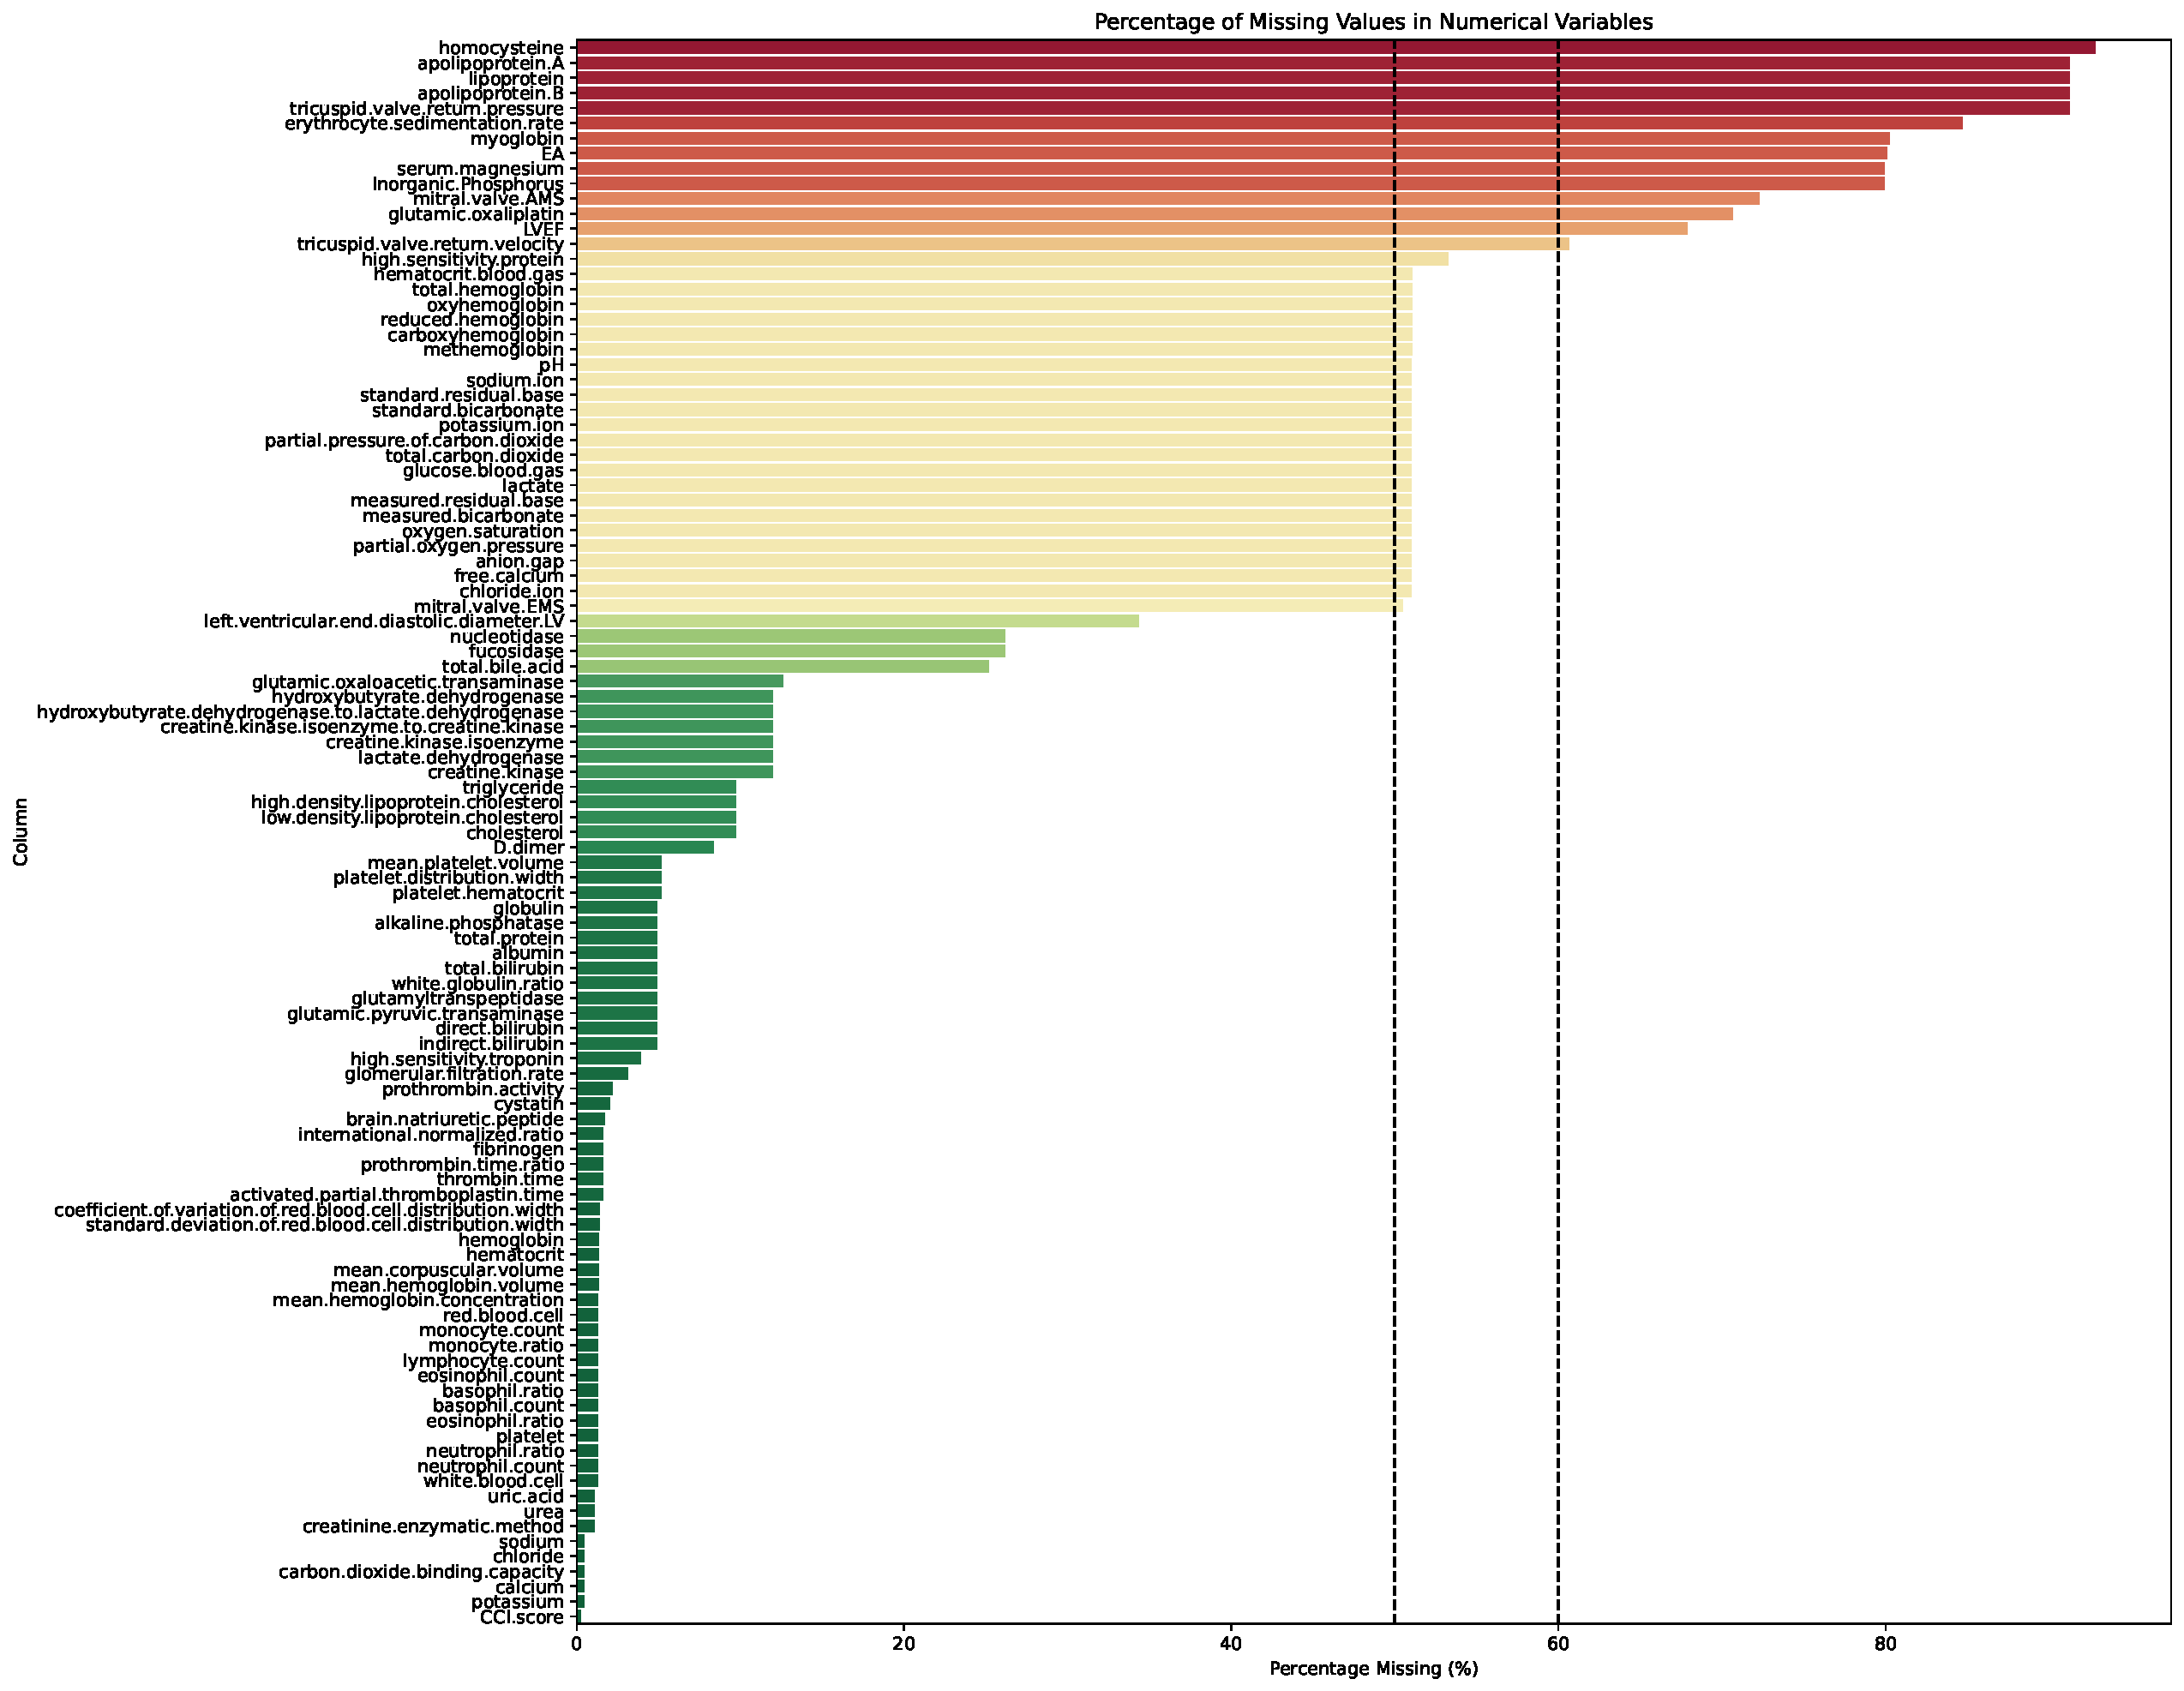
\includegraphics[width=3.1in]{missing_values_percentages.pdf}
%     \caption{Percentage of missing values.}
%     \label{fig:missing-values}
% \end{figure}

All 14 variables with over 60\% missing were discarded, while for those with 50\% to 60\% missing we computed whether there was any variable in the sub-50\% missing part of the dataset with more than 0.80 correlation. If that was the case, we discarded them: 9 variables were removed.

Finally, among the remaining ones in the 50\% to 60\% missing range we computed the correlation matrix, clustered with hierarchical clustering, with the aim of seeing a clearer block structure, see \autoref{fig:clustered-correlation-matrix}. With this techniques we discarded 3 more variables.

\begin{figure}[htpb]
    \centering
    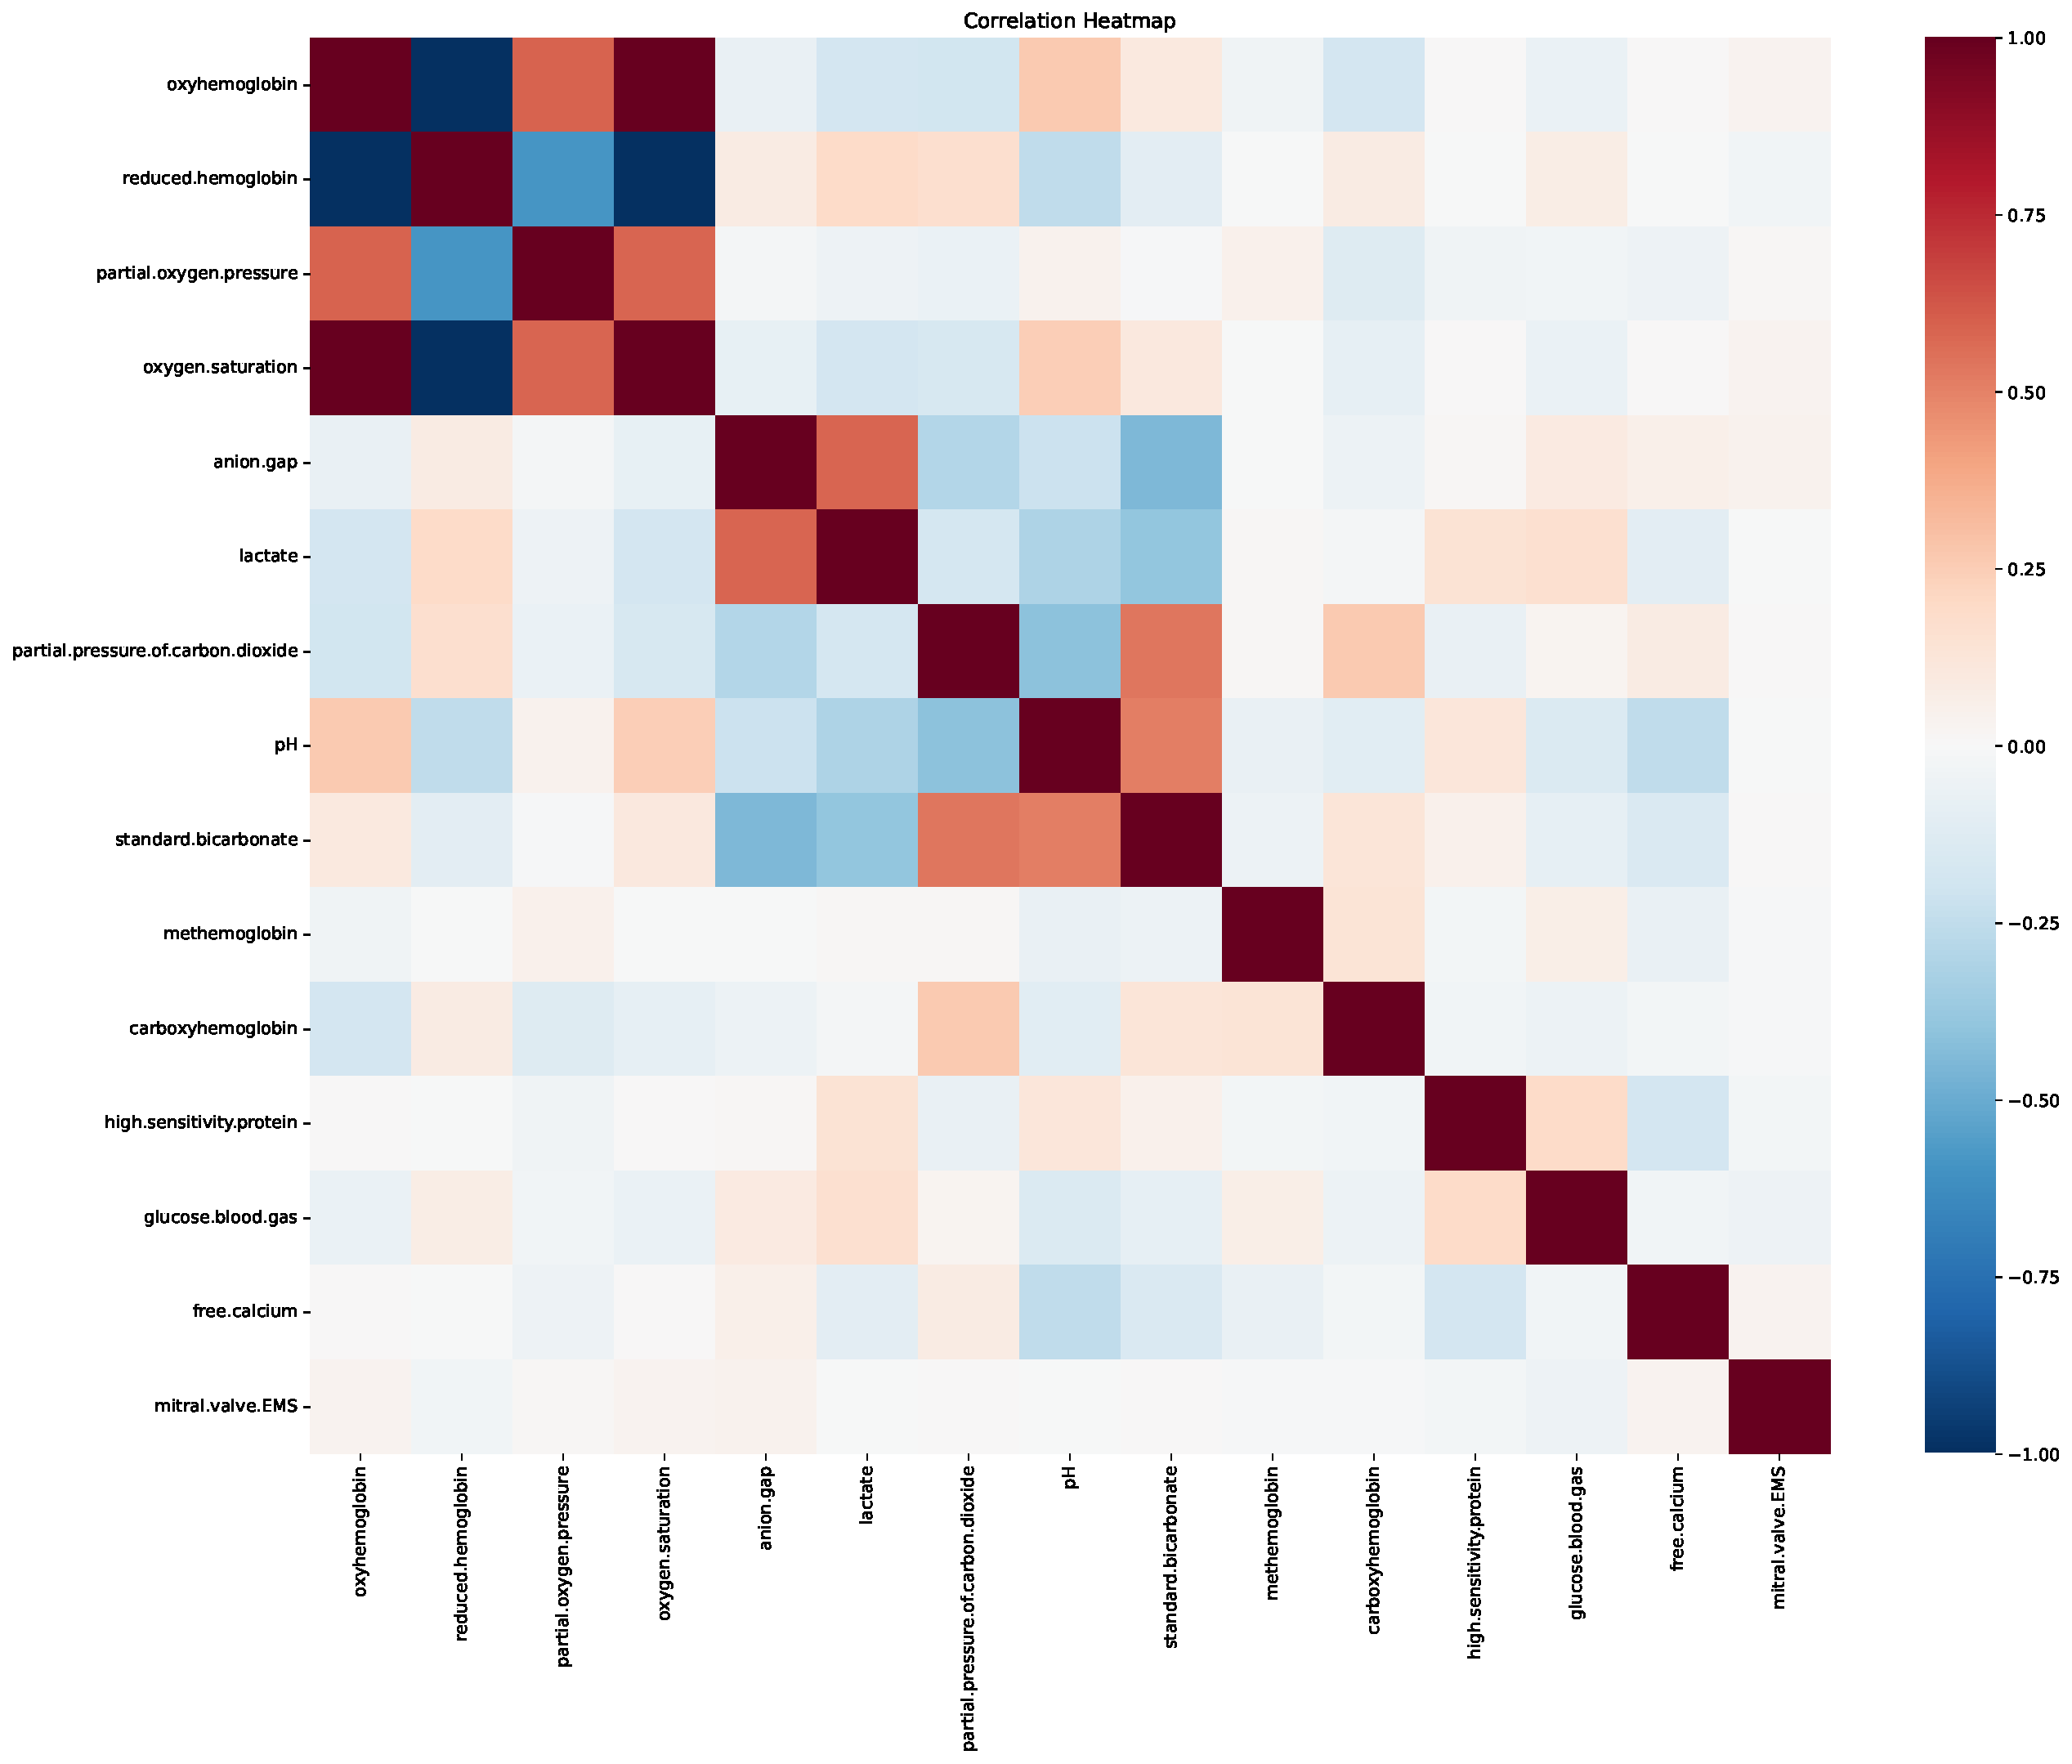
\includegraphics[width=3.1in]{clustered_correlation_matrix.pdf}
    \caption{Correlation matrix of variables with 50\%-60\% missing values.}
    \label{fig:clustered-correlation-matrix}
\end{figure}

\subsubsection{Outlier analysis}\label{sec:outlier-analysis}

An overall histogram of all numerical variables made very clear that there were many outliers in the data.

The approach we followed was to identify them and judge one by one whether or not the values were physiologically possible or not, by checking the literature. In that case, instead of discarding the patient completely, we set the value to NaN to impute it later. During the approach we tried to be as conservative as possible to retain as much information as possible, but simultaneously give to the models high quality data that would enable good separation.

Outliers were identified by calculating the sample $Z$-score of each variable:
\begin{align*}
    Z\text{-score} = \frac{X-\bar{X}}{s}
\end{align*}
where $\bar{X}$ is the sample mean and $s$ is the sample standard deviation.

A threshold of 3 or above was applied to detect them, depending on the specific variable.

After this procedure, there were still three variables that showed possible outliers: \texttt{eosinophil.count}, \texttt{high.sensitivity.troponin} and \texttt{glutamic.pyruvic.transaminase}. However, these variables were marked by many models as important, so we decided to keep them anyway without changes. We suspect there may have been discordances in inserting the values, i.e. for some patients with some unit of measure, for other patients with another unit. We strongly recommend double checking these variables.

\subsubsection{Removing low variance variables}

Among the categorical variables, we removed 16 variables with more than 95\% dominance in values counts, while for the numerical variables we removed 2 constant ones.

\subsubsection{Correlation analysis}

Using clinical knowledge, we inspected some groups of variables we thought could be quite correlated, then we proceeded with discarding variables with more than 0.85 correlation with the others, ultimately removing 12 more variables.

Up to this point, 62 variables had been discarded.

\subsection{Modeling}

The dataset was split according to an 85:15 train-test ratio, preserving the target proportions, and part of the training was designated to validation set.

%All statistical analyses were carried out using Python and mainly the Scikit-learn\footcite{scikit-learn} library.

\subsubsection{Preprocessing categorical data}

Categorical variables were encoded using one-hot encoding.

\subsubsection{Preprocessing numerical data}

Numerical variables were imputed using a KNN imputer with 5 neighbours and then standardized for letting the training converge.

\subsubsection{Class imbalance}

The dataset was a bit imbalanced, with 39.6\% of observations belonging to class 1 (positives). To tackle the problem, whenever the model allowed for it, we passed class weights based on the inverse of percentage of samples over the total.

\subsubsection{Performance indexes}

The main metric used to compare models was the \gls{auc} under the \gls{roc} curve.

\subsection{Feature selection}

Ideally we wanted to perform a backward selection. However, since the initial number of features is 131, the process is very computationally intensive (about 20 seconds per feature to be removed) and greedy, so we would risk discarding important variables too soon. To speed up the process we developed the following method:

\begin{itemize}
    \item Train a \gls{lr} with strong $L^1$ penalty to select a set $S_\text{LR}$ of features.
    \item Train a \gls{rf} and create an $S_\text{RF}$ set of features made by the top 30 features by impurity decrease importance.
    \item Create a set $S_\text{reduced} = S_\text{LR} \cup S_\text{RF}$. The reason for this is that the way \gls{lr} and \gls{rf} select variables is very different, in fact the intersection $S_\text{LR} \cap S_\text{RF}$ was very small. In this way we take advantage of both.
\end{itemize}

We could now perform a backward selection based on this $S_\text{reduced}$ set of features, and inspecting the evolution of the \gls{auc} we selected a suitable number of features $S^\star_1$. Then, since the results are often different, we performed a forward selection from 0 to 10 features on the same model to get the set $S^\star_2$, and finally we took the union of the two as our final features set $S^\star = S^\star_1 \cup S^\star_2$ of 13 variables.

For visualization purposes, in \autoref{fig:distribution-target} we plotted the KDE of some features in $S^\star$ separately with the respect to the target.

It's really clear the difference in distribution of the \texttt{creatinine.enzymatic.method}, we expect it to be important in the final model.

\begin{figure}
    \centering
    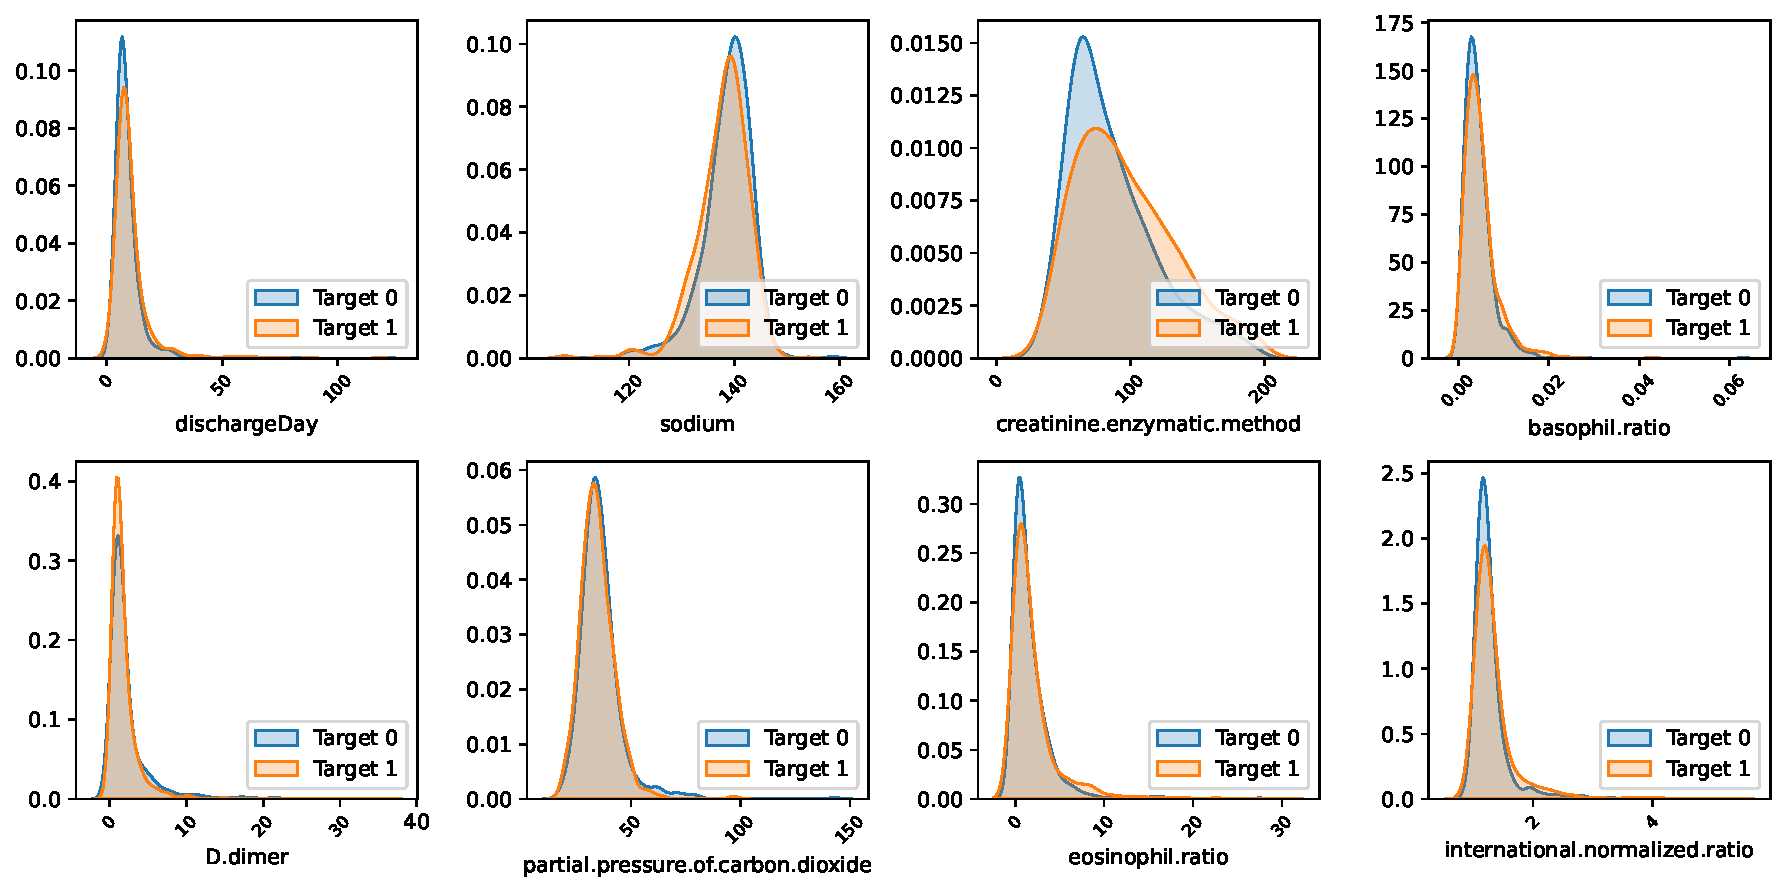
\includegraphics[width=3.1in]{distribution_wrt_target.pdf}
    \caption{Distribution with the respect to the target of sodium and creatinine enzymatic method.}
    \label{fig:distribution-target}
\end{figure}

\subsubsection{Model selection}

We trained 6 different classifiers on the unscaled selected features with a 5-fold stratified cross-validation to tune the hyperparameters.
Besides those, we made an attempt with an SVM, but the training failed to converge except on the scaled data (which makes interpretability harder) and didn't perform well, therefore we don't include it.
